\documentclass{article}
\usepackage[scale=.91]{geometry}
\usepackage[svgnames]{xcolor}
\usepackage{tikz}
\usetikzlibrary{penrose}
%
% 81 thin rhombi, 147 thick rhombi
%
\thispagestyle{empty}
\pagestyle{empty}
\pgfmathsetmacro\cphi{(sqrt(5)+1)/2}
\pgfmathsetmacro\sphi{sin(36)}
\pgfmathsetmacro\chphi{2*cos(18)}
\pgfmathsetmacro\shphi{sin(18)}
\colorlet{thinRhombus}{DarkOrchid}
\colorlet{thickRhombus}{DarkSlateGray}
\colorlet{circleArc}{RosyBrown}
\colorlet{longArc}{LawnGreen}

\colorlet{kite}{HotPink}
\colorlet{dart}{Fuchsia}

\begin{document}
\end{document}
\begin{tikzpicture}[
  scale=3,
  every Penrose tile/.style={
    transform shape,
  },
  every kite/.style={
    draw=black,
    ultra thick,
    fill=kite,
  },
  every dart/.style={
    draw=black,
    ultra thick,
    fill=dart,
  },
  every circle arc/.style={
    line width=1mm,
    draw=circleArc
  },
  every long arc/.style={
    line width=2mm,
    draw=longArc
  }
]
\pic[kite,name=a];
\pic[kite,align with=a along a];
\pic[kite,align with=a along A];
\pic[dart,align with=a along b];
\pic[dart,align with=a along B];
\begin{scope}[xshift=4cm]
\pic[dart,name=a];
\pic[kite,align with=a along a];
\pic[kite,align with=a along A];
\pic[kite,align with=a along b];
\pic[kite,align with=a along B];
\end{scope}
\end{tikzpicture}


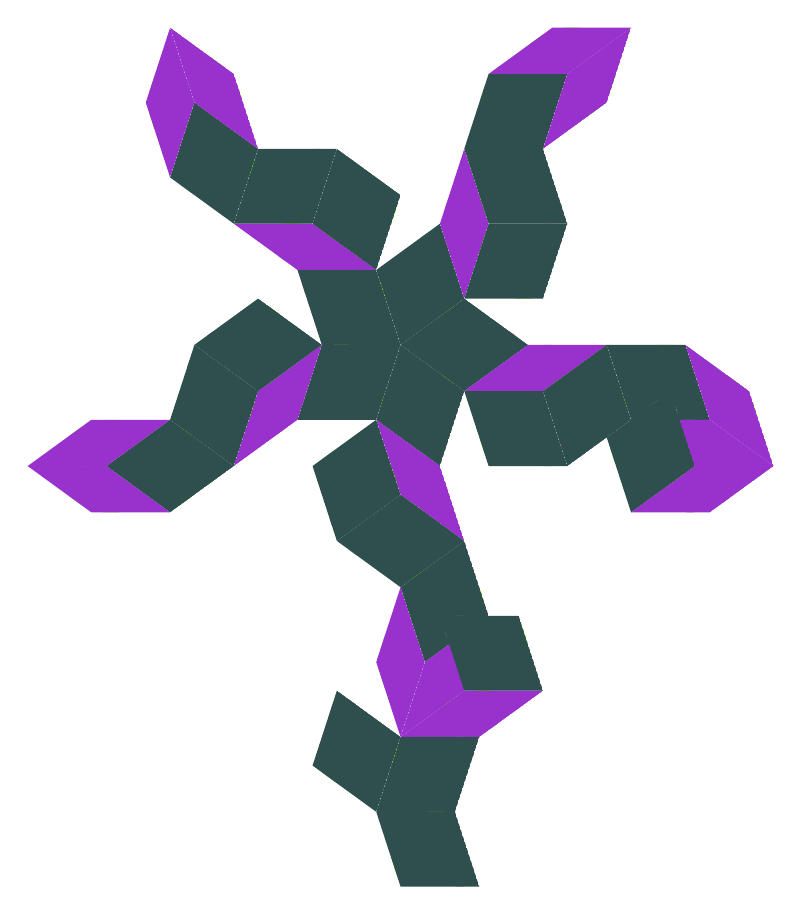
\begin{tikzpicture}[
  scale=3,
  rotate=-18,
  every Penrose tile/.style={
    transform shape,
  },
  every rhombus/.style={
    draw=black,
    ultra thick,
  },
  every thin rhombus/.style={
    fill=thinRhombus,
  },
  every thick rhombus/.style={
    fill=thickRhombus,
  },
  every circle arc/.style={
    line width=1mm,
    draw=circleArc
  },
  every long arc/.style={
    line width=2mm,
    draw=longArc
  }
]
\pic[thick rhombus,name=a0];
\foreach[evaluate=\k as \kmo using int(\k-1)] \k in {1,...,4} 
{
  \pic[thick rhombus,name=a\k,align with={a\kmo} along B];
}
\foreach \k in {0,...,4} 
{
  \pic[thin rhombus,name=b\k,align with={a\k} along A];
  \pic[thick rhombus,name=c\k,align with={b\k} along B];
  \pic[thick rhombus,name=d\k,align with={b\k} along b];
  \pic[thick rhombus,name=e\k,align with={c\k} along B];
  \foreach \l/\a in {{0/a},{1/A}}
    \pic[thin rhombus,name=f\k\l,align with={e\k} along \a];
}
\pic[thin rhombus,name=g0,align with={f40} along b];
\pic[thin rhombus,name=g1,align with={f01} along B];
\foreach \l/\a in {{0/b},{1/B}}
  \pic[thick rhombus,name=h\l,align with={g\l} along \a];
\pic[thick rhombus,name=i,align with=g0 along A];
\foreach \l/\a in {{0/b},{1/B}}
  \pic[thick rhombus,name=j\l,align with=i along \a];
\end{tikzpicture}


\end{document}
